\title{Circuitos Eléctricos}
\maketitle
\section*{fuentes de tensión - ideal}
\justifying
Una fuente de tensión continua produce una tensión constante en la carga,	independientemente de lo grande o pequeña que sea la resistencia de carga.

Solo varia la corriente de carga cuando varia la resistencia de carga.

\begin{figure}[h]
	\centering
	\subfloat[Esquema]{
		\label{f:Esquema}
		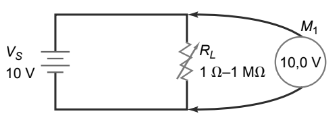
\includegraphics[width=0.2\textwidth]{f_t_c_esquema}}
	\subfloat[Grafica]{
		\label{f:Grafica}
		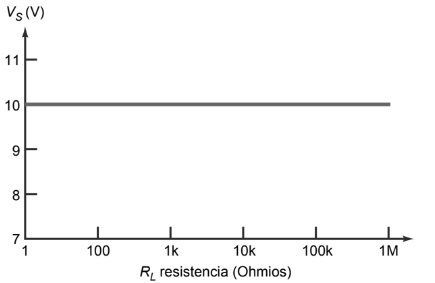
\includegraphics[width=0.2\textwidth]{f_t_c_grafica}}
	\label{f:Fuente de tension - Ideal}
\end{figure}

\section*{fuentes de tensión - real}
\justifying
Una fuente de tensión ideal es un dispositivo teórico; no puede existir en la naturaleza, porque cuando la resistencia de carga tiende a cero, la corriente por la carga tiende a infinito.

En este caso, la tensión en la carga no se aproxima al valor ideal hasta que la resistencia de
carga es mucho mayor que la resistencia de la fuente.

\centering{Fuente de tension continua $\rightarrow$ $R_s$ $<$ $0,01R_L$}

\section*{fuentes de corriente - ideal}
\justifying
Una fuente de corriente continua ideal, genera una corriente constante en la carga para distintas resistencias de carga

\section*{conversiones de fuentes}
\justifying
Es importante darse cuenta que la equivalencia entre una fuente de corriente y una fuente de tension existe solo en sus terminales externos.

Las caracteristicas internas de cada una son muy diferentes.

\section*{fuentes de corriente en paralelo}
\justifying
Dos o mas fuentes de corriente en paralelo pueden reemplazarse por una sola fuente de corriente de magnitud, determinada por la diferencia de la suma de la corrientes en una direccion y la suma en la direccion opuesta.

La nueva resistencia interna en paralelo es la resistencia total de los elementos resistivos en paralelo.
\section*{fuentes de corriente en serie}
\justifying
La corriente a traves de cada rama de una red solo puede tener un valor

Teniendo esto en cuenta, al conectar diferentes fuentes corriente en serie, la corriente que sale de un punto, sera diferente que la entra al otro, por lo cual es una situación imposible segun la Ley de Kirchhoff de las corrientes de un nodo.
\section*{divisor de corriente}
\justifying
La corriente que pasa por la resitencia es igual a la corriente total por la resistencia de la otra rama, dividido la suma de las resistencias de las dos ramas.
\begin{figure}[h]
	\centering
	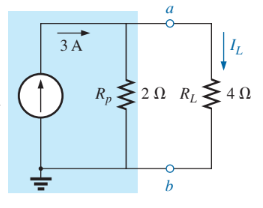
\includegraphics[width=0.5\linewidth]{imagenes/screenshot001}
	\label{fig:screenshot001}
\end{figure}

\centering $ I_L = I \dfrac{R_p}{R_p + R_L} $ ;
\centering $ I_p = I \dfrac{R_L}{R_p + R_L} $ ;
\centering $ V = I \dfrac{R_p R_L}{R_p + R_L} $

\section*{divisor de tension}
\justifying
La caida de tension de la resistencia es igual al voltaje aplicado, por la resistencia en la que se quiere calcular, dividido la suma de las dos resistencias.
\begin{figure}[h]
	\centering
	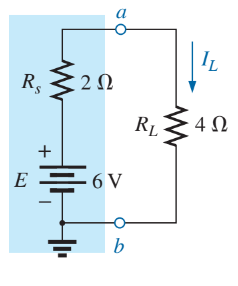
\includegraphics[width=0.4\linewidth]{imagenes/screenshot002}
	\label{fig:screenshot002}
\end{figure}

\centering $ V_L = E \dfrac{R_L}{R_L + R_s} $ ;
\centering $ V_s = E \dfrac{R_s}{R_L + R_s} $ 
\section*{metodo de corriente de mallas - formato}
\begin{itemize}
	\justifying
	\item Asigne una corriente de lazo a cada lazo cerrado independiente en el sentido 
	de las manecillas del rejoj.
	\item El numero de ecuaciones requerias es igual al numero de lazos independientes
	cerrados seleccionado. La columna 1 de cada ecuacion se forma fumando los valores de
	resistencia de los resistores a traves de los cuales pasa la corriente de lazo de interes y multiplicando el resutado por dicha corriente de lazo.
	\item Ahora tenemos que considerar los terminos mutuos, los cuales, como se observo en los ejemplos anteriores, siempre se restan de la primera columna. Un termino mutuo es simplemente cualquier elemento resistivo a traves del cual pasa una corriente de lazo adicional.
	
	Es posible tenermas de un termino mutuo si la corriente de lazo de interes tiene un elemento en comun con otra corriente mas de lazo.
	
	Cada termino es el producto del resistor mutuo por la otra corriente de lazo que pasa a traves del mismo elemento.
	\item La columna a la derecha del signo igual es la suma algebraica de las fuentes de voltaje a traves de los cuales pasa la corriente de lazo de interes. Se asigna signos positivos a la fuentes de voltaje cuya polaridad es tal que la corriente de lazo pasa de la terminal negativa a la positiva.
	\item Resuelva las ecuaciones simultaneas resustantes para las corrientes de lazo deseadas.
\end{itemize}
Ejemplo
\begin{figure}[h]
	\centering
	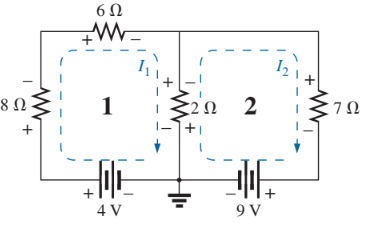
\includegraphics[width=0.4\linewidth]{imagenes/screenshot003}
	\label{fig:screenshot003}
\end{figure}
\[
\left \{
\begin{array}{rr}
	(8 \Omega + 6 \Omega + 2 \Omega) I_1 - 2 \Omega I_2  =& 4 V \\
	(2 \Omega + 7 \Omega) I_2 - 2\Omega I_1 =& -9 V \\
\end{array}
\right .
\]
\section*{metodo de voltajes de nodos - formato}
\begin{itemize}
	\justifying
	\item Seleccione un nodo de referencia, y asigne una etiqueta de voltaje subindexado a los (N-1) nodos restante de la red.
	\item El numero de ecuaciones de voltajes subindexados (N-1). La columna 1 de cada ecuacion se forma sumando las conductancias vinculadas al nodo de interes y multiplicando el resutado por dicho voltaje nodal subindexado.
	\item Ahora consideramos los terminos mutuos, los cuales, como se señalo en el ejemplo anterior, siempre se restan de la primera columna.
	
	Es posible tener mas de un termino mutuio si el voltaje nodal de interes tiene un elemento en comun con mas de otro voltaje nodal.
	
	Cada termino mituo es el producto de la conductancia mutua por el otro voltaje nodal, vinculado a dicha conductancia.
	\item La columna a la derecha del signo igual es la suma algebraica de la fuente de corriente vinculada al nodo de interes. A una fuente de corriente se le asigna un signo positivo si suministra corriente a un nodo y un signo negativo si extrae corriente de el.
	\item Resuelva las ecuaciones simultaneas resutantes para los voltajes deseados. 
\end{itemize}
Ejemplo
\begin{figure}
	\centering
	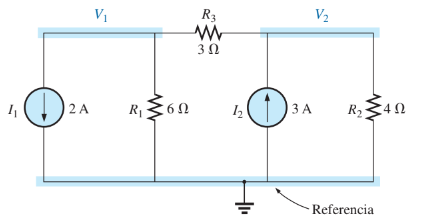
\includegraphics[width=0.7\linewidth]{imagenes/screenshot004}
	\label{fig:screenshot004}
\end{figure}
\[
\left \{
\begin{array}{rr}
	\left( \dfrac{1}{6 \Omega + 3 \Omega + 2 \Omega} \right)  V_1 - \dfrac{1}{3 \Omega} V_2  =& - 2 A \\\\
	\left( \dfrac{1}{3 \Omega + 4 \Omega } \right) V_2 - \dfrac{1}{3 \Omega} V_1 =& 3 A
\end{array}
\right .
\]
\section*{teorema de superposicion}
\section*{teorema de thevenin}
\section*{teorema de norton}